% Options for packages loaded elsewhere
\PassOptionsToPackage{unicode}{hyperref}
\PassOptionsToPackage{hyphens}{url}
%
\documentclass[
  12pt,
]{article}
\usepackage{amsmath,amssymb}
\usepackage{lmodern}
\usepackage{iftex}
\ifPDFTeX
  \usepackage[T1]{fontenc}
  \usepackage[utf8]{inputenc}
  \usepackage{textcomp} % provide euro and other symbols
\else % if luatex or xetex
  \usepackage{unicode-math}
  \defaultfontfeatures{Scale=MatchLowercase}
  \defaultfontfeatures[\rmfamily]{Ligatures=TeX,Scale=1}
\fi
% Use upquote if available, for straight quotes in verbatim environments
\IfFileExists{upquote.sty}{\usepackage{upquote}}{}
\IfFileExists{microtype.sty}{% use microtype if available
  \usepackage[]{microtype}
  \UseMicrotypeSet[protrusion]{basicmath} % disable protrusion for tt fonts
}{}
\makeatletter
\@ifundefined{KOMAClassName}{% if non-KOMA class
  \IfFileExists{parskip.sty}{%
    \usepackage{parskip}
  }{% else
    \setlength{\parindent}{0pt}
    \setlength{\parskip}{6pt plus 2pt minus 1pt}}
}{% if KOMA class
  \KOMAoptions{parskip=half}}
\makeatother
\usepackage{xcolor}
\IfFileExists{xurl.sty}{\usepackage{xurl}}{} % add URL line breaks if available
\IfFileExists{bookmark.sty}{\usepackage{bookmark}}{\usepackage{hyperref}}
\hypersetup{
  pdftitle={Supplementary Information},
  hidelinks,
  pdfcreator={LaTeX via pandoc}}
\urlstyle{same} % disable monospaced font for URLs
\usepackage[margin = 1.0in]{geometry}
\usepackage{graphicx}
\makeatletter
\def\maxwidth{\ifdim\Gin@nat@width>\linewidth\linewidth\else\Gin@nat@width\fi}
\def\maxheight{\ifdim\Gin@nat@height>\textheight\textheight\else\Gin@nat@height\fi}
\makeatother
% Scale images if necessary, so that they will not overflow the page
% margins by default, and it is still possible to overwrite the defaults
% using explicit options in \includegraphics[width, height, ...]{}
\setkeys{Gin}{width=\maxwidth,height=\maxheight,keepaspectratio}
% Set default figure placement to htbp
\makeatletter
\def\fps@figure{htbp}
\makeatother
\setlength{\emergencystretch}{3em} % prevent overfull lines
\providecommand{\tightlist}{%
  \setlength{\itemsep}{0pt}\setlength{\parskip}{0pt}}
\setcounter{secnumdepth}{-\maxdimen} % remove section numbering
\usepackage{times} % Times New Roman font
\usepackage[T1]{fontenc}

\usepackage[none]{hyphenat}

\usepackage{setspace}
\doublespacing
\setlength{\parskip}{1em}

\usepackage{lineno}
\renewcommand{\linenumberfont}{\normalfont\tiny}

\usepackage{pdfpages}

\usepackage{indentfirst}

\usepackage[labelsep=period, labelfont=bf]{caption}
\renewcommand{\thefigure}{S\arabic{figure}}
\renewcommand{\figurename}{Supplementary Figure}
\renewcommand{\thetable}{S\arabic{table}}
\renewcommand{\tablename}{Supplementary Table}
\captionsetup{justification=raggedright,singlelinecheck=false}

\usepackage{pdflscape}
\newcommand{\blandscape}{\begin{landscape}}
\newcommand{\elandscape}{\end{landscape}}

\usepackage{siunitx}
\DeclareSIUnit\molar{\mole\per\cubic\deci\metre}
\DeclareSIUnit\Molar{\textsc{m}}
\DeclareSIUnit\cells{\text{cells}}

\usepackage{caption}
\captionsetup{justification=justified}

\usepackage{float}

\usepackage{txfonts}

\renewcommand{\figureautorefname}{Fig.}

\usepackage{microtype}
\usepackage{booktabs}
\usepackage{longtable}
\usepackage{array}
\usepackage{multirow}
\usepackage{wrapfig}
\usepackage{float}
\usepackage{colortbl}
\usepackage{pdflscape}
\usepackage{tabu}
\usepackage{threeparttable}
\usepackage{threeparttablex}
\usepackage[normalem]{ulem}
\usepackage{makecell}
\usepackage{xcolor}
\ifLuaTeX
  \usepackage{selnolig}  % disable illegal ligatures
\fi

\title{\textbf{Supplementary Information}}
\usepackage{etoolbox}
\makeatletter
\providecommand{\subtitle}[1]{% add subtitle to \maketitle
  \apptocmd{\@title}{\par {\large #1 \par}}{}{}
}
\makeatother
\subtitle{\textbf{Temporal variation in the prokaryotic community of a
nearshore marine environment}}
\author{}
\date{\vspace{-2.5em}}

\begin{document}
\maketitle

\vspace{10mm}

Marino Korlević\textsuperscript{1\(*\)}, Marsej
Markovski\textsuperscript{1}, Gerhard J. Herndl\textsuperscript{2,3},
and Mirjana Najdek\textsuperscript{1}

1. Center for Marine Research, Ruđer Bošković Institute, Croatia

2. Department of Functional and Evolutionary Ecology, University of
Vienna, Austria

3. Department of Marine Microbiology and Biogeochemistry, Royal
Netherlands Institute for Sea Research (NIOZ), Utrecht University, The
Netherlands

\textsuperscript{\(*\)}To whom correspondence should be addressed:

Marino Korlević

G. Paliaga 5, 52210 Rovinj, Croatia

Tel.: +385 52 804 768

Fax: +385 52 804 780

e-mail:
\href{mailto:marino.korlevic@irb.hr}{\nolinkurl{marino.korlevic@irb.hr}}

\newpage
\sisetup{mode = text}
\setlength\parindent{24pt}

\hypertarget{supplementary-figures}{%
\subsection{Supplementary figures}\label{supplementary-figures}}

\begin{figure}[H]

{\centering 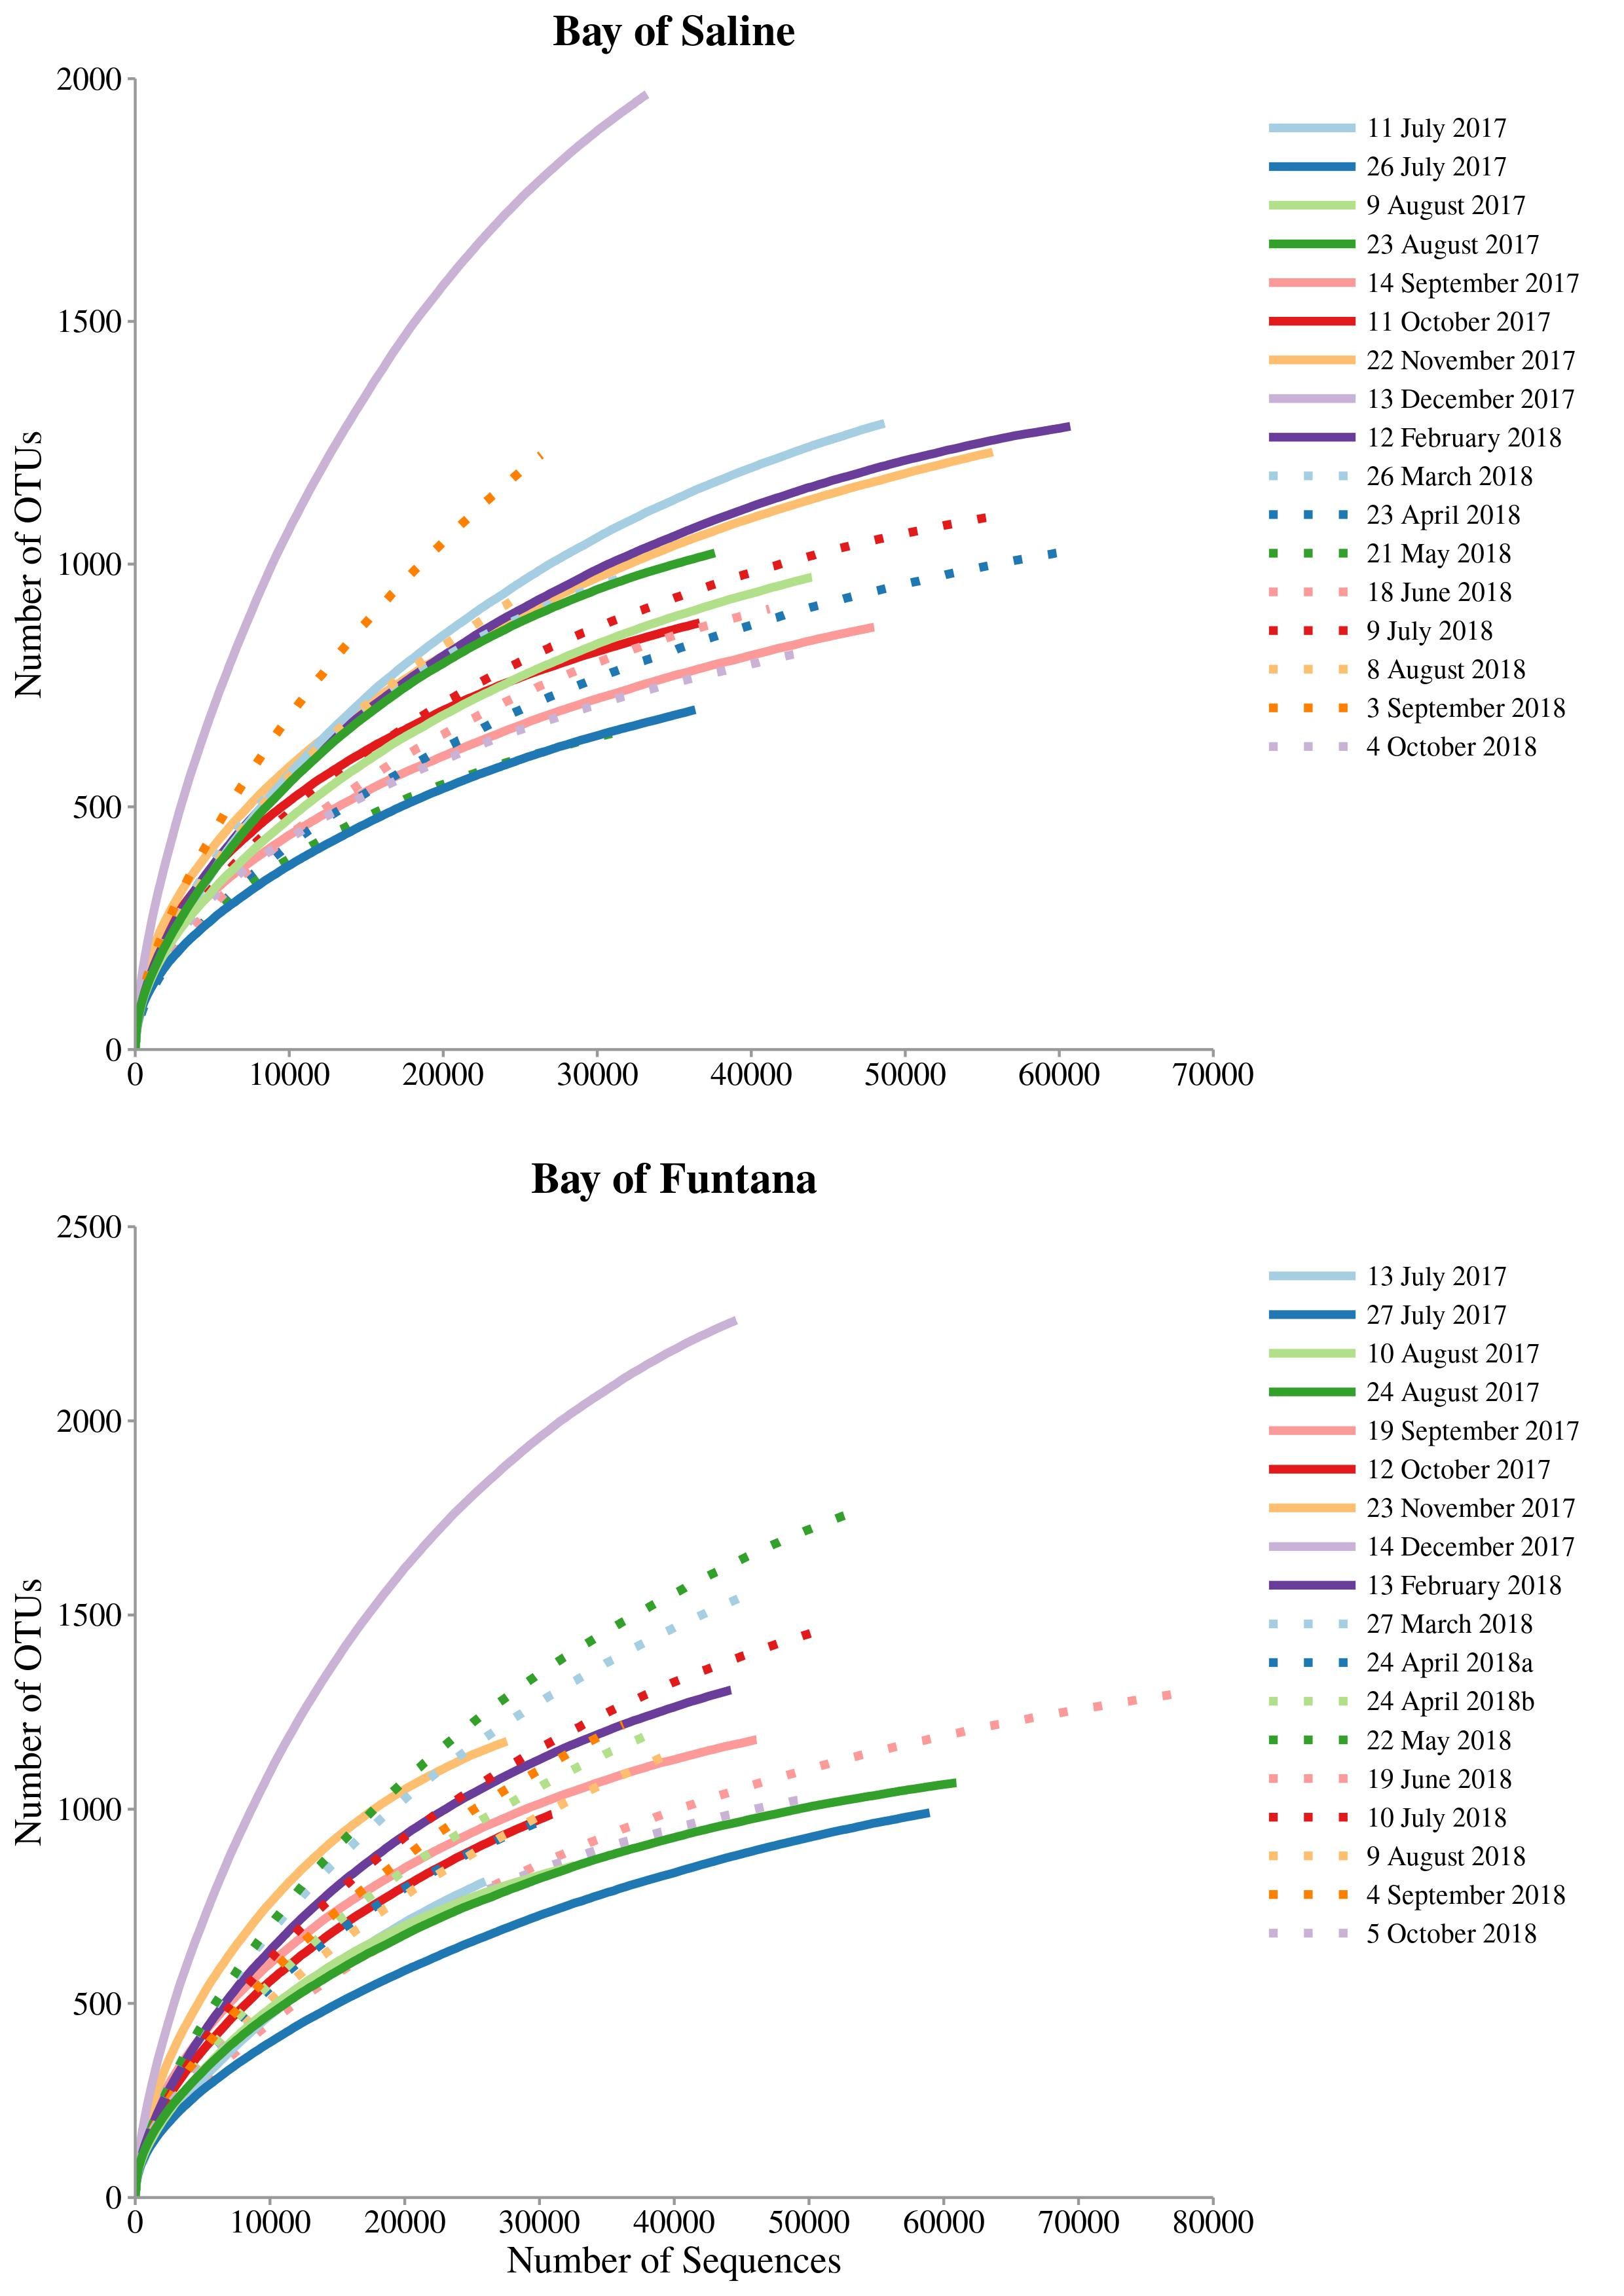
\includegraphics[width=0.85\linewidth]{../results/figures/rarefaction} 

}

\caption{Rarefaction curves of bacterial and archaeal communities sampled in the Bay of Saline and Funtana.\label{rarefaction}}\label{fig:unnamed-chunk-1}
\end{figure}

\begin{figure}[H]

{\centering 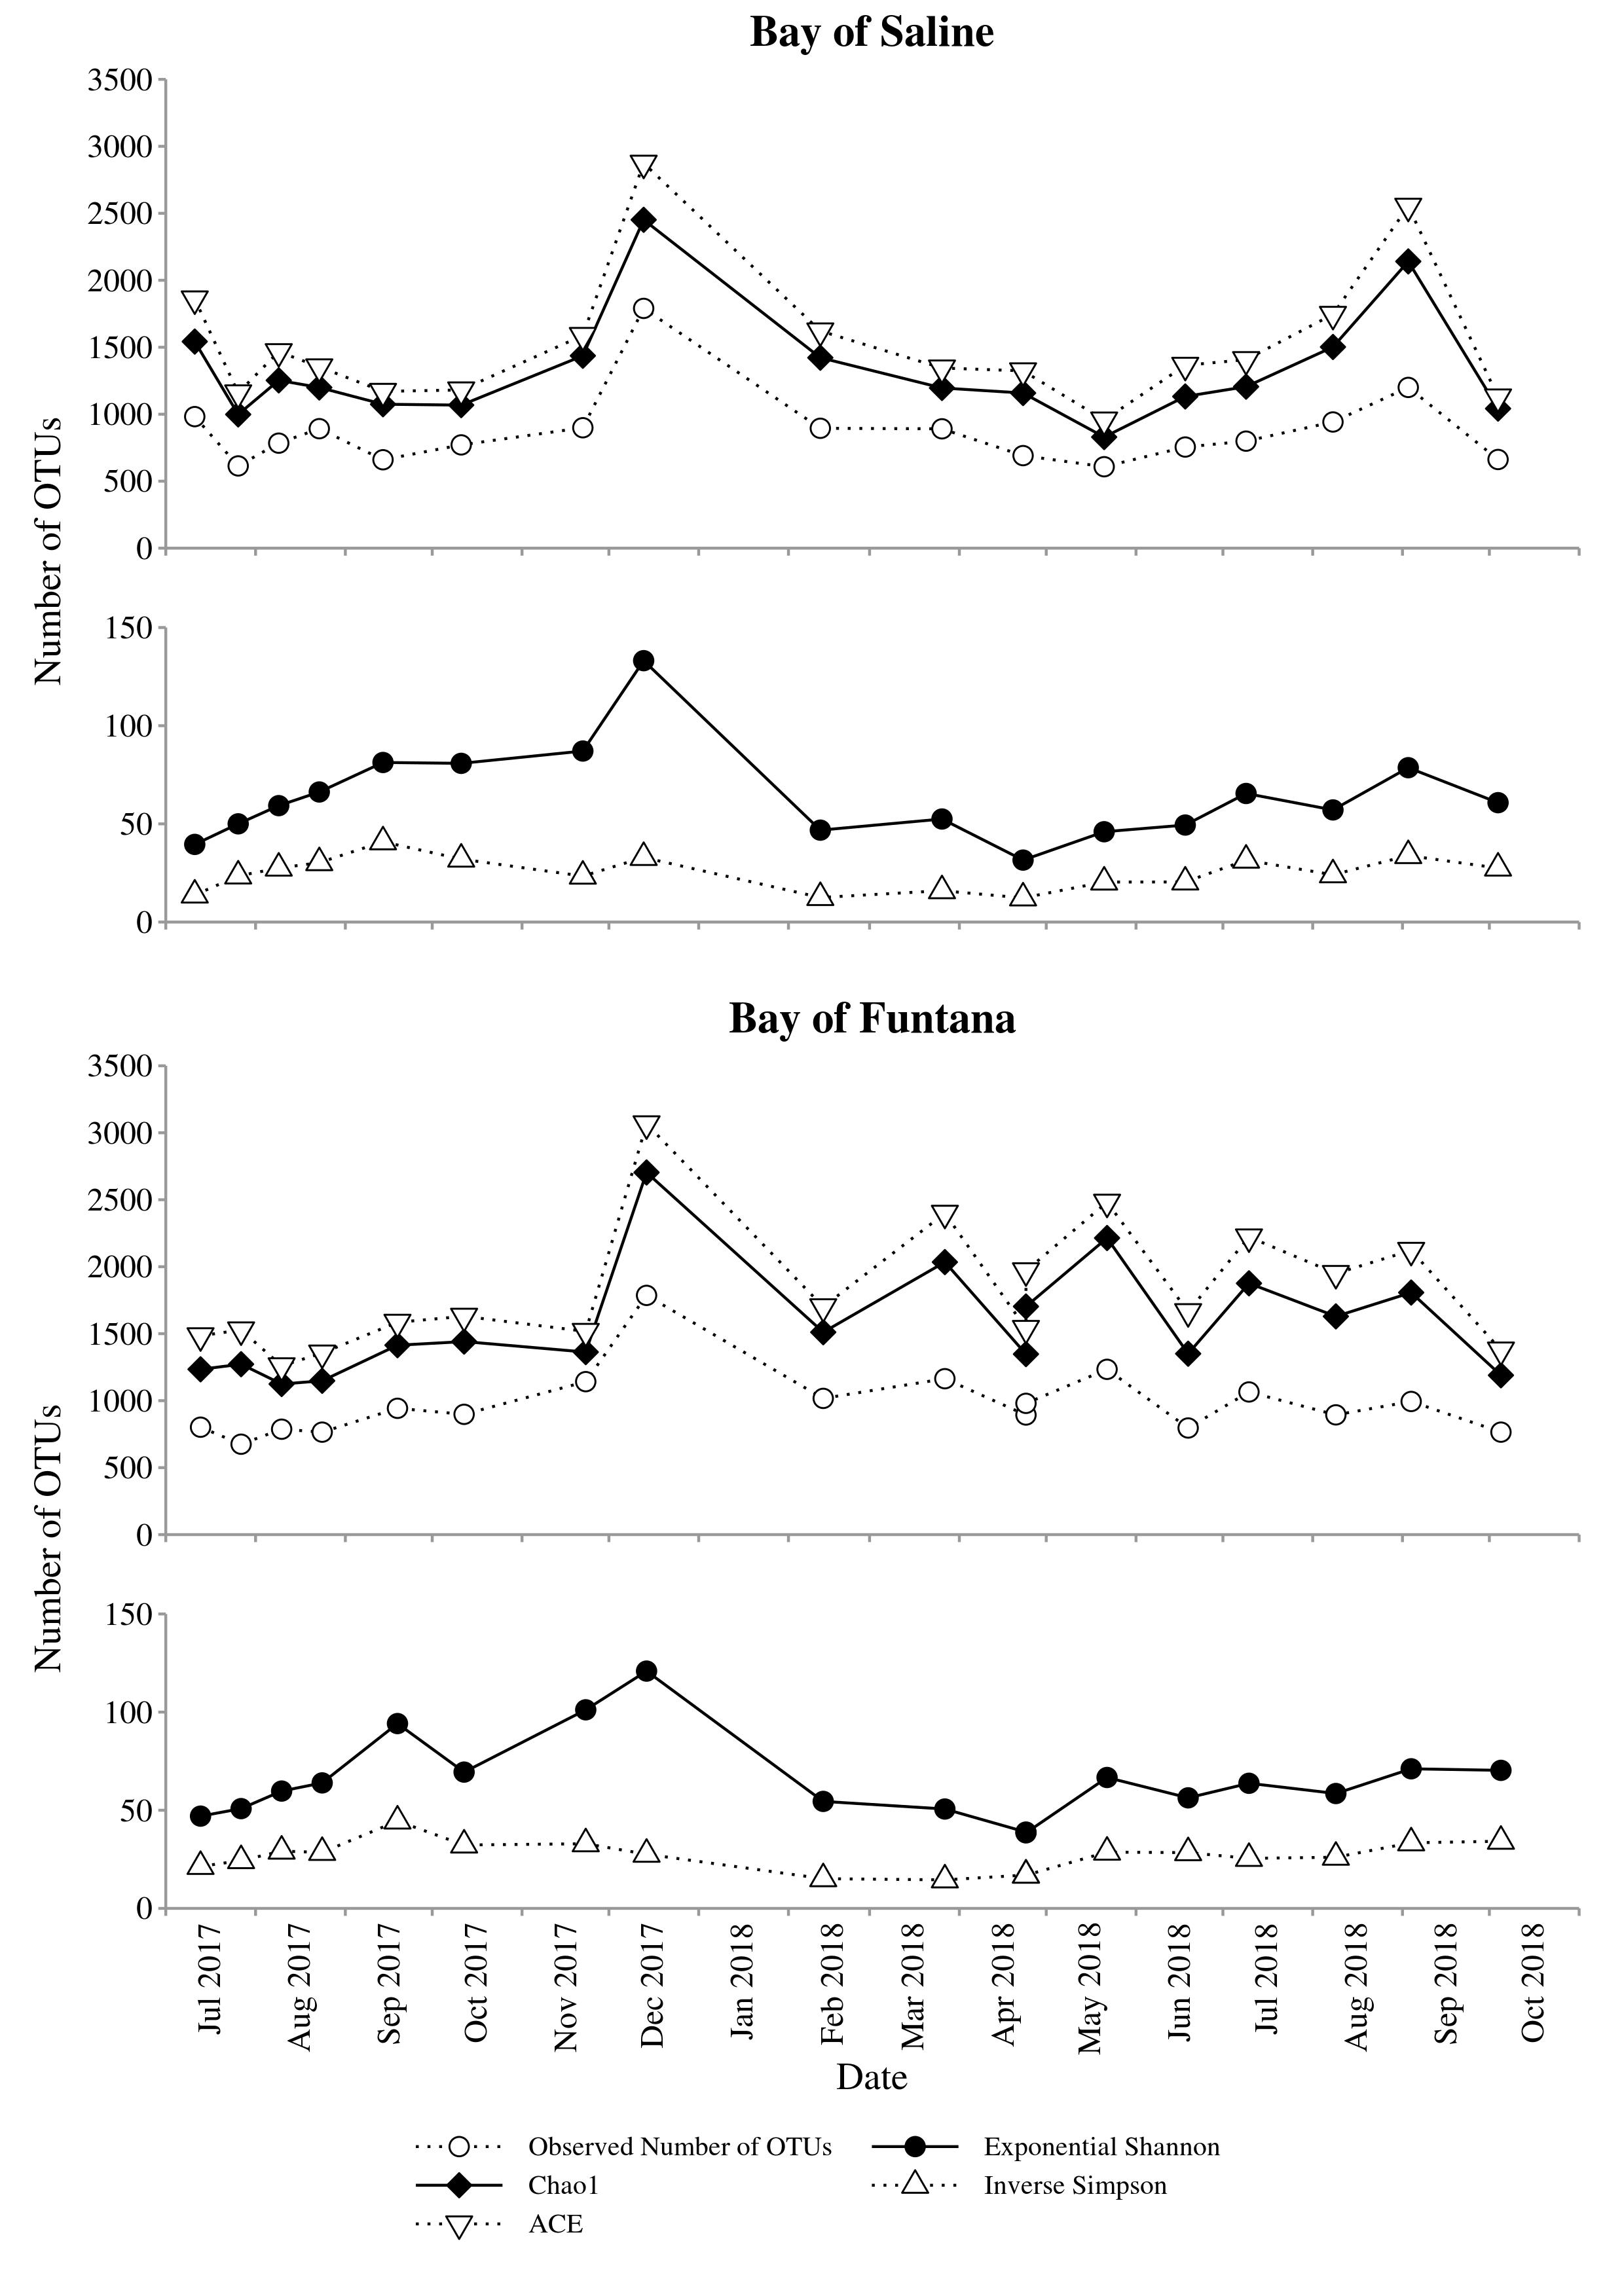
\includegraphics[width=0.85\linewidth]{../results/figures/calculators} 

}

\caption{Seasonal dynamics of observed number of OTUs, Chao1, ACE, exponential of the Shannon diversity index, and Inverse Simpson index of bacterial and archaeal communities sampled in the Bay of Saline and Funtana.\label{calculators}}\label{fig:unnamed-chunk-2}
\end{figure}

\begin{figure}[H]

{\centering 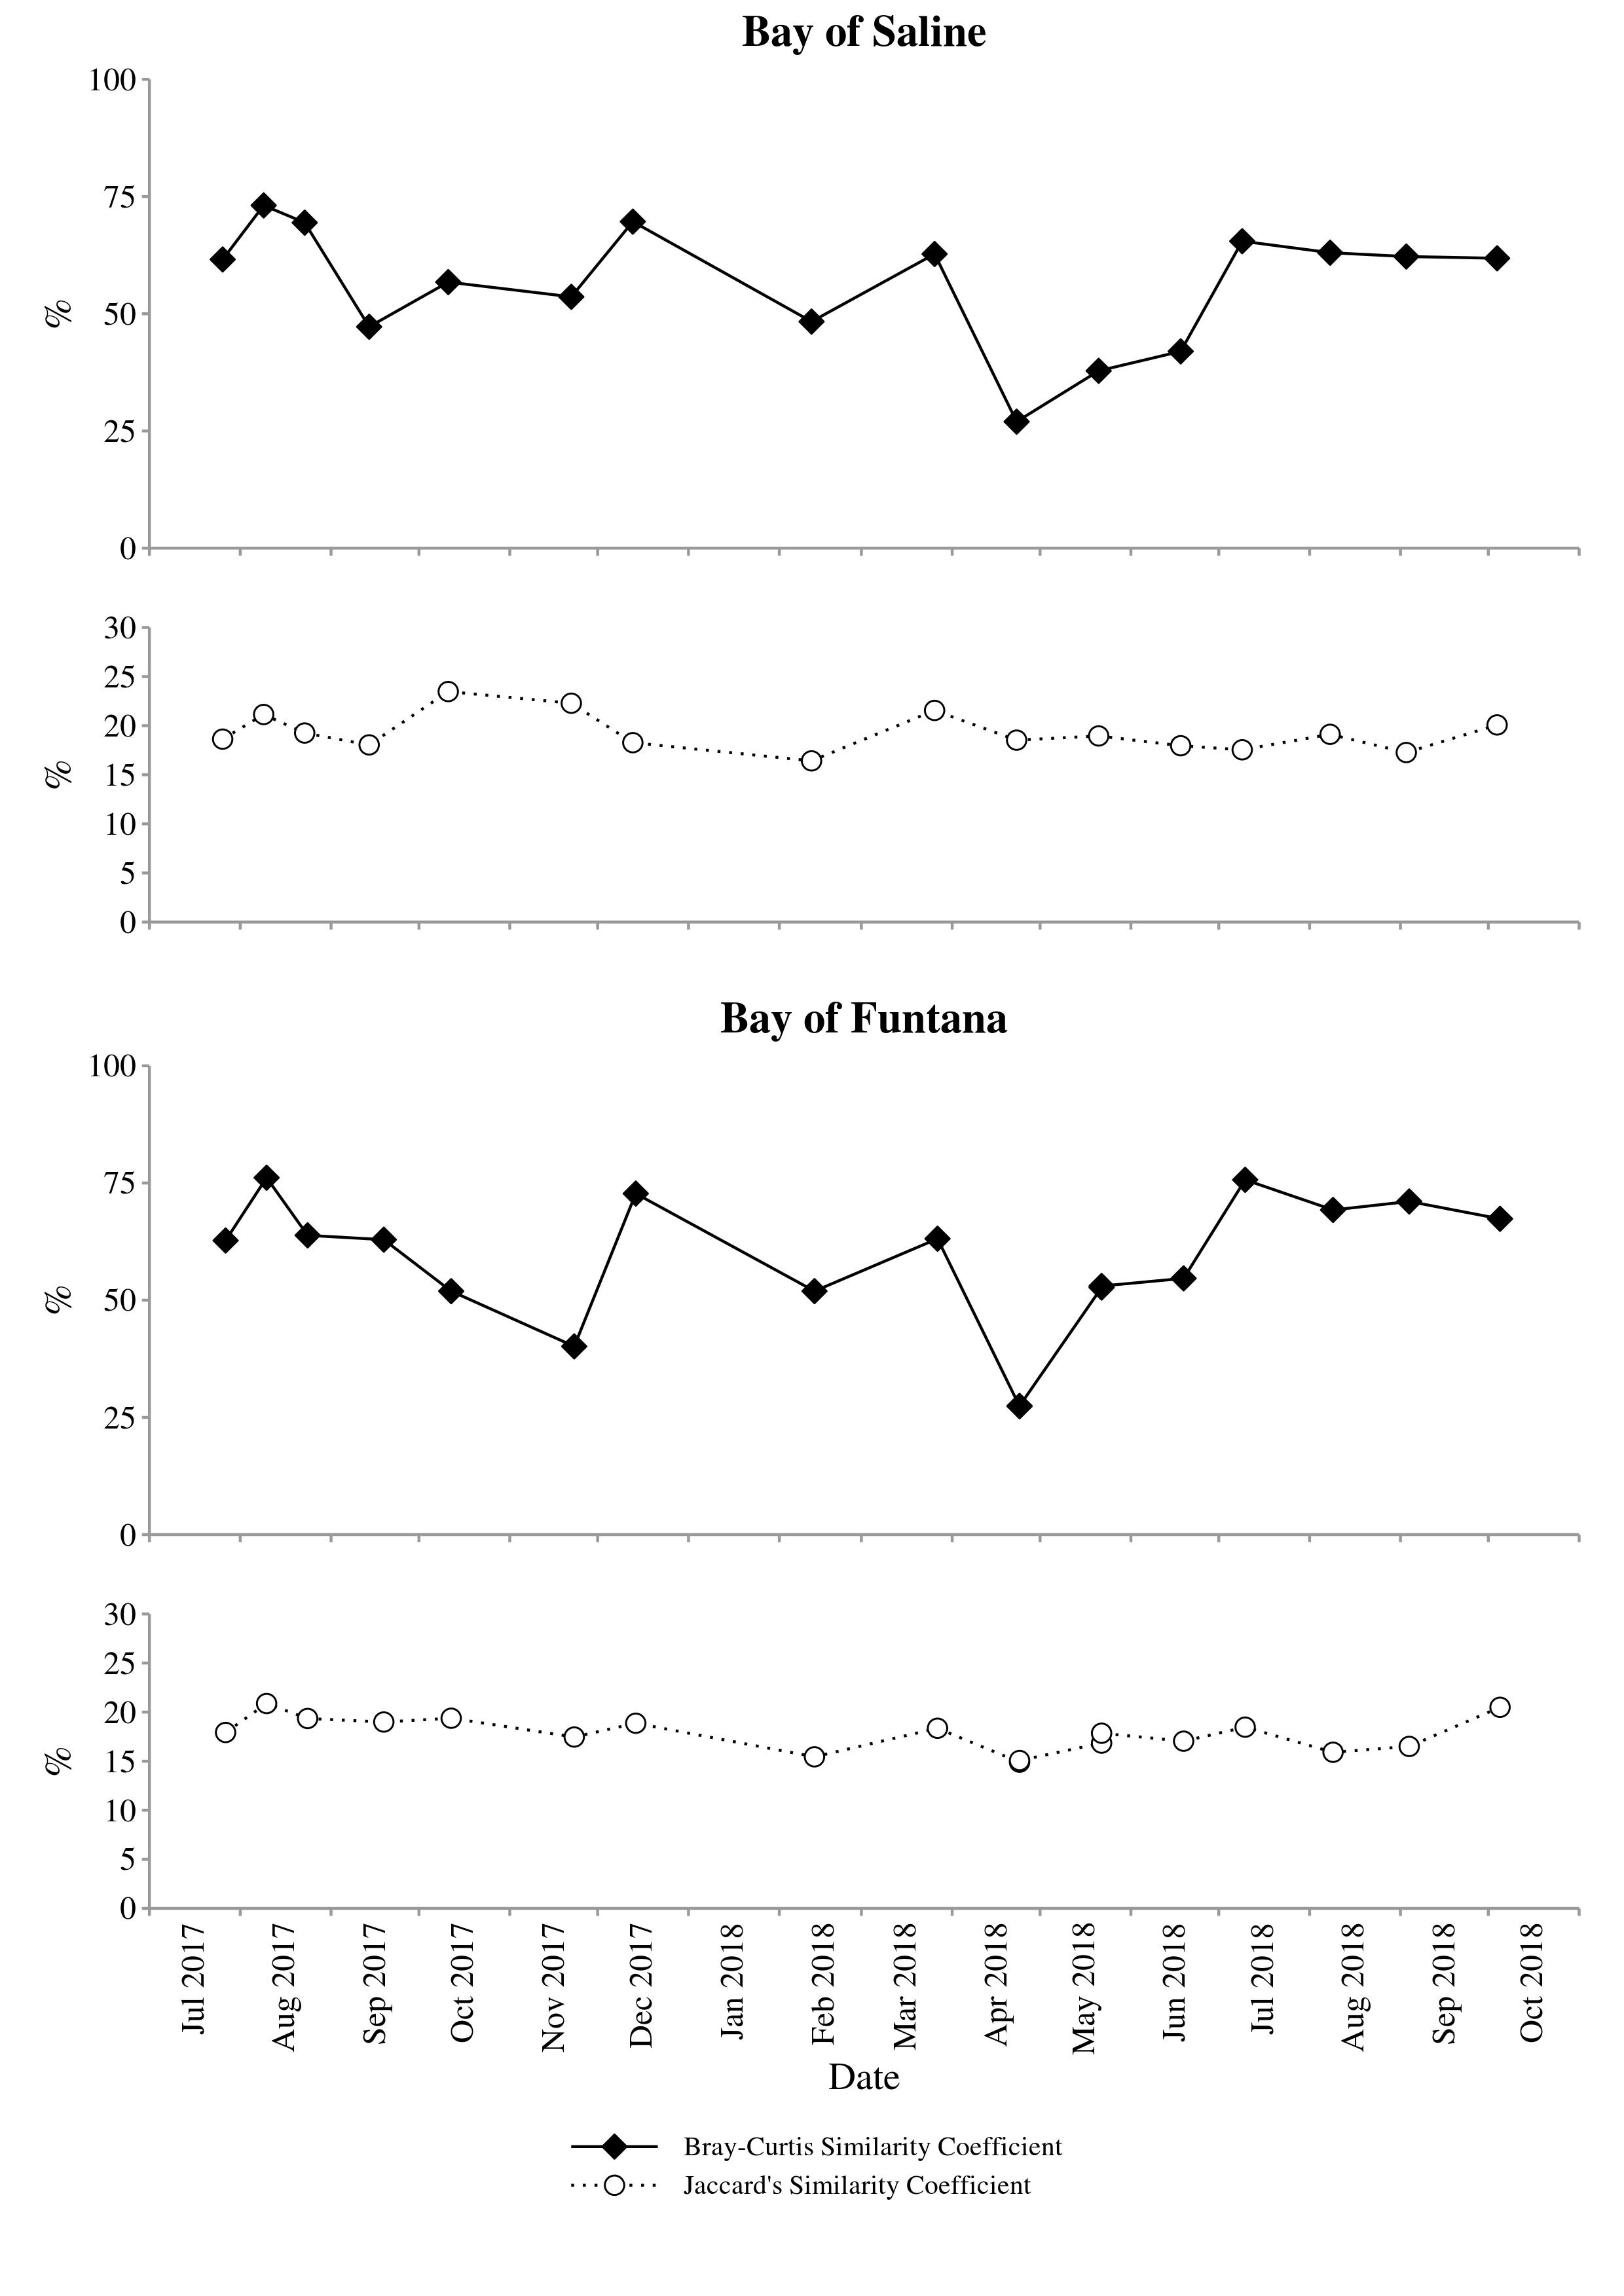
\includegraphics[width=0.85\linewidth]{../results/figures/seasonal_shared} 

}

\caption{Proportion of shared bacterial and archaeal communities (Bray-Curtis similarity coefficient) and shared bacterial and archaeal OTUs (Jaccard's similarity coefficient) between consecutive sampling dates of communities sampled in the Bay of Saline and Funtana.\label{shared}}\label{fig:unnamed-chunk-3}
\end{figure}

\newpage

\hypertarget{supplementary-table}{%
\subsection{Supplementary table}\label{supplementary-table}}

\begingroup\fontsize{9}{11}\selectfont

\begin{longtable}[t]{>{\centering\arraybackslash}p{6em}cccc}
\caption{\label{tab:nseq_notus}Sample ID, sampling station and date, and number of sequences and OTUs of each sample. The number of sequences and OTUs was calculated after exclusion of sequences without known relatives (no relative sequences) and eukaryotic, chloroplast, and mitochondrial sequences.\label{nseq_notus}}\\
\toprule
\textbf{Sample ID} & \textbf{Station} & \textbf{Date} & \textbf{Number of Sequences} & \textbf{Number of OTUs}\\
\midrule
\endfirsthead
\caption[]{Sample ID, sampling station and date, and number of sequences and OTUs of each sample. The number of sequences and OTUs was calculated after exclusion of sequences without known relatives (no relative sequences) and eukaryotic, chloroplast, and mitochondrial sequences.\label{nseq_notus} \textit{(continued)}}\\
\toprule
\textbf{Sample ID} & \textbf{Station} & \textbf{Date} & \textbf{Number of Sequences} & \textbf{Number of OTUs}\\
\midrule
\endhead

\endfoot
\bottomrule
\endlastfoot
2 & Bay of Saline & 11 July 2017 & 48,652 & 1,290\\
3 & Bay of Funtana & 13 July 2017 & 25,989 & 814\\
4 & Bay of Saline & 26 July 2017 & 36,368 & 700\\
5 & Bay of Funtana & 27 July 2017 & 58,952 & 991\\
6 & Bay of Saline & 9 August 2017 & 43,934 & 973\\
7 & Bay of Funtana & 10 August 2017 & 32,624 & 855\\
8 & Bay of Saline & 23 August 2017 & 37,636 & 1,023\\
9 & Bay of Funtana & 24 August 2017 & 60,937 & 1,068\\
10 & Bay of Saline & 14 September 2017 & 47,977 & 870\\
11 & Bay of Funtana & 19 September 2017 & 46,110 & 1,179\\
12 & Bay of Saline & 11 October 2017 & 36,655 & 879\\
13 & Bay of Funtana & 12 October 2017 & 30,930 & 987\\
14 & Bay of Saline & 22 November 2017 & 55,678 & 1,231\\
15 & Bay of Funtana & 23 November 2017 & 27,586 & 1,175\\
16 & Bay of Saline & 13 December 2017 & 33,229 & 1,968\\
17 & Bay of Funtana & 14 December 2017 & 44,602 & 2,259\\
18 & Bay of Saline & 12 February 2018 & 60,714 & 1,284\\
19 & Bay of Funtana & 13 February 2018 & 44,215 & 1,307\\
20 & Bay of Saline & 26 March 2018 & 31,953 & 975\\
21 & Bay of Funtana & 27 March 2018 & 46,359 & 1,566\\
22 & Bay of Saline & 23 April 2018 & 60,343 & 1,026\\
23a & Bay of Funtana & 24 April 2018 & 30,979 & 982\\
23b & Bay of Funtana & 24 April 2018 & 38,573 & 1,200\\
24 & Bay of Saline & 21 May 2018 & 32,232 & 660\\
25 & Bay of Funtana & 22 May 2018 & 53,875 & 1,773\\
26 & Bay of Saline & 18 June 2018 & 41,180 & 908\\
27 & Bay of Funtana & 19 June 2018 & 77,466 & 1,298\\
28 & Bay of Saline & 9 July 2018 & 56,739 & 1,104\\
29 & Bay of Funtana & 10 July 2018 & 50,803 & 1,460\\
30 & Bay of Saline & 8 August 2018 & 25,360 & 942\\
31 & Bay of Funtana & 9 August 2018 & 39,058 & 1,133\\
32 & Bay of Saline & 3 September 2018 & 26,355 & 1,225\\
33 & Bay of Funtana & 4 September 2018 & 36,211 & 1,217\\
34 & Bay of Saline & 4 October 2018 & 43,955 & 823\\
35 & Bay of Funtana & 5 October 2018 & 49,573 & 1,026\\*
\end{longtable}
\endgroup{}

\newpage
\blandscape
\begingroup\fontsize{9}{11}\selectfont

\begin{longtable}[t]{>{\centering\arraybackslash}m{8em}ccl}
\caption{\label{tab:core_otus_taxonomy_table}Taxonomic classification of OTUs present at every sampling date at each station (Bay of Saline and Funtana). Only ten OTUs with the highest number of sequences after normalization to the minimum number of reads per sample are shown.\label{core_otus_taxonomy_table}}\\
\toprule
\textbf{Station} & \textbf{OTU Number} & \textbf{No. of Sequences} & \textbf{OTU Taxonomy}\\
\midrule
\endfirsthead
\caption[]{Taxonomic classification of OTUs present at every sampling date at each station (Bay of Saline and Funtana). Only ten OTUs with the highest number of sequences after normalization to the minimum number of reads per sample are shown.\label{core_otus_taxonomy_table} \textit{(continued)}}\\
\toprule
\textbf{Station} & \textbf{OTU Number} & \textbf{No. of Sequences} & \textbf{OTU Taxonomy}\\
\midrule
\endhead

\endfoot
\bottomrule
\endlastfoot
 & Otu00001 & 33741 & \textit{Bacteria}; \textit{Proteobacteria}; \textit{Alphaproteobacteria}; SAR11 Clade; Subclade I; Subclade Ia\\
\nopagebreak
 & Otu00002 & 27922 & \textit{Bacteria}; \textit{Proteobacteria}; \textit{Alphaproteobacteria}; \textit{Rhodospirillales}; AEGEAN-169 Marine Group\\
\nopagebreak
 & Otu00003 & 19674 & \textit{Bacteria}; \textit{Cyanobacteria}; \textit{Cyanobacteriia}; \textit{Synechococcales}; \textit{Cyanobiaceae}; \textit{Synechococcus}\\
\nopagebreak
 & Otu00004 & 19220 & \textit{Bacteria}; \textit{Proteobacteria}; \textit{Alphaproteobacteria}; SAR11 Clade; Subclade III\\
\nopagebreak
 & Otu00005 & 17607 & \textit{Bacteria}; \textit{Proteobacteria}; \textit{Alphaproteobacteria}; SAR11 Clade; Subclade II\\
\nopagebreak
 & Otu00006 & 16140 & \textit{Bacteria}; \textit{Proteobacteria}; \textit{Gammaproteobacteria}; SAR86 Clade\\
\nopagebreak
 & Otu00007 & 12760 & \textit{Bacteria}; \textit{Proteobacteria}; \textit{Gammaproteobacteria}; \textit{Oceanospirillales}; \textit{Litoricolaceae}; \textit{Litoricola}\\
\nopagebreak
 & Otu00008 & 10799 & \textit{Bacteria}; \textit{Bacteroidota}; \textit{Bacteroidia}; \textit{Flavobacteriales}; \textit{Cryomorphaceae}; uncultured \textit{Cryomorphaceae}\\
\nopagebreak
 & Otu00011 & 9709 & \textit{Bacteria}; \textit{Bacteroidota}; \textit{Bacteroidia}; \textit{Flavobacteriales}; \textit{Flavobacteriaceae}; NS5 Marine Group\\
\nopagebreak
\multirow{-10}{8em}{\centering\arraybackslash Bay of Saline} & Otu00012 & 7800 & \textit{Bacteria}; \textit{Proteobacteria}; \textit{Gammaproteobacteria}; \textit{Cellvibrionales}; \textit{Halieaceae}; OM60 Clade\\
\cmidrule{1-4}\pagebreak[0]
 & Otu00001 & 30081 & \textit{Bacteria}; \textit{Proteobacteria}; \textit{Alphaproteobacteria}; SAR11 Clade; Subclade I; Subclade Ia\\
\nopagebreak
 & Otu00002 & 25323 & \textit{Bacteria}; \textit{Proteobacteria}; \textit{Alphaproteobacteria}; \textit{Rhodospirillales}; AEGEAN-169 Marine Group\\
\nopagebreak
 & Otu00003 & 20920 & \textit{Bacteria}; \textit{Cyanobacteria}; \textit{Cyanobacteriia}; \textit{Synechococcales}; \textit{Cyanobiaceae}; \textit{Synechococcus}\\
\nopagebreak
 & Otu00004 & 19157 & \textit{Bacteria}; \textit{Proteobacteria}; \textit{Alphaproteobacteria}; SAR11 Clade; Subclade III\\
\nopagebreak
 & Otu00008 & 16312 & \textit{Bacteria}; \textit{Bacteroidota}; \textit{Bacteroidia}; \textit{Flavobacteriales}; \textit{Cryomorphaceae}; uncultured \textit{Cryomorphaceae}\\
\nopagebreak
 & Otu00005 & 16166 & \textit{Bacteria}; \textit{Proteobacteria}; \textit{Alphaproteobacteria}; SAR11 Clade; Subclade II\\
\nopagebreak
 & Otu00010 & 16096 & \textit{Bacteria}; \textit{Proteobacteria}; \textit{Alphaproteobacteria}; \textit{Rhodobacterales}; \textit{Rhodobacteraceae}; \textit{Ascidiaceihabitans}\\
\nopagebreak
 & Otu00007 & 14847 & \textit{Bacteria}; \textit{Proteobacteria}; \textit{Gammaproteobacteria}; \textit{Oceanospirillales}; \textit{Litoricolaceae}; \textit{Litoricola}\\
\nopagebreak
 & Otu00006 & 12451 & \textit{Bacteria}; \textit{Proteobacteria}; \textit{Gammaproteobacteria}; SAR86 Clade\\
\nopagebreak
\multirow{-10}{8em}{\centering\arraybackslash Bay of Funtana} & Otu00011 & 9972 & \textit{Bacteria}; \textit{Bacteroidota}; \textit{Bacteroidia}; \textit{Flavobacteriales}; \textit{Flavobacteriaceae}; NS5 Marine Group\\*
\end{longtable}
\endgroup{}
\elandscape

\end{document}
